\documentclass{article}
\usepackage[utf8]{inputenc}

\title{CTA200H, RV Fitting Project}
\author{Gurman Sachdeva \\ 1007896314}
\date{May 16, 2022}
\usepackage{amsmath,amscd,amssymb,amsfonts,amsthm}
\usepackage[shortlabels]{enumitem}
\usepackage{array}
\usepackage{geometry}
\geometry{letterpaper, portrait, margin=1in}
\usepackage{graphicx}
\usepackage{caption}
\usepackage{hyperref}
\usepackage{siunitx}

\newcommand{\for}{\texttt{for}}
\newcommand{\rebound}{\texttt{REBOUND}}
\newcommand{\simf}{\texttt{q2\_simulate}}

\begin{document}
\maketitle

%%%%%%%%%%%%%%%%%%%%%%%%%%%%%%%%%%%%%%%%%%%%%%%%%%%%%%%%%%%%%%%%%%%%%%%
\section*{Introduction}

This document describes the goals of the project notebook and the methods by which these goals are achieved. The notebook contains full solutions for questions 1, 2, 3.1, and 3.2. 

This project intends to explore the radial velocity curve of an exoplanetary system, and what this curve can say about the orbital parameters of planets in the system. In the notebook, we first cover the steps involved in using \rebound{} to simulate an N-body system, then experiment with orbital parameters in 2-body systems to see their effects on the radial velocity curve of the host star, and finally compare a model radial velocity curve generated from such a simulation to measured radial velocity data of the exoplanetary system HD155358. 

\newpage
%%%%%%%%%%%%%%%%%%%%%%%%%%%%%%%%%%%%%%%%%%%%%%%%%%%%%%%%%%%%%%%%%%%%%%%

\section{Using \rebound}
We first import the required libraries; rebound, matplotlib and numpy. A simulation is initialized with the prescribed units, planets, and orbital parameters, and integrated for 500 years using a \for{} loop such that the data of each planet can be stored in an array at every time interval. \\

The plot of the orbital trajectories of both planets is shown in \ref{fig:q1f1}, where Planet 1 is the higher mass planet. We observe that both planets have slightly elliptical orbits (with semi-major axis parallel to the y-axis of the plot). Moreover, the whole system migrates towards the positive y-direction due to the nature of the simulation, since both planets begin with momentum in the positive y-direction, which is nearly exactly preserved through integration. 

\begin{figure}[htp]
    \centering
    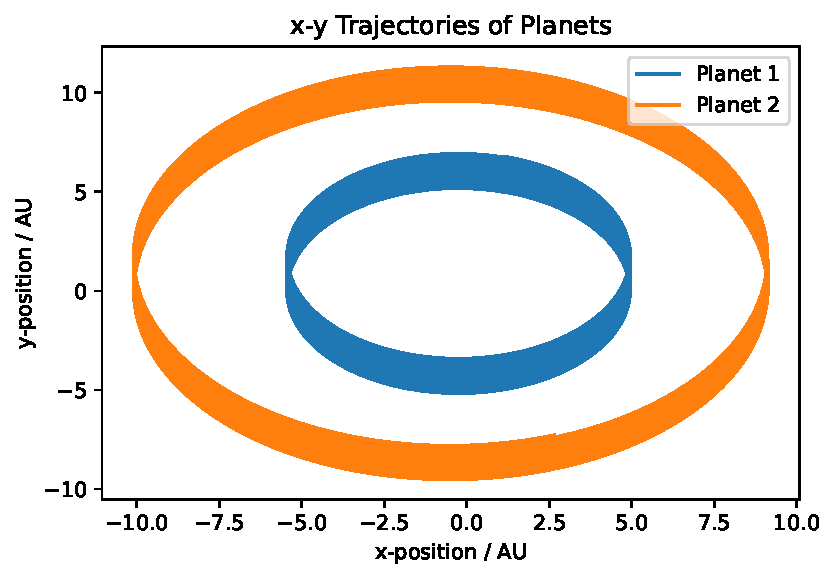
\includegraphics[width=0.6\textwidth]{q1f1.pdf}
    \captionsetup{justification=centering}
    \caption{The orbital trajectories of both planets in the first \rebound{} simulation.}
    \label{fig:q1f1}
\end{figure}

\newpage

Figure \ref{fig:q1f2} below shows the evolution of the semi-major axis of Planet 1 as a function of time. We see that it exhibits several concurrent frequencies of oscillation due its gravitational interactions with the other planet and the star. This hints at the ability for a star's RV curve to reveal a wealth of information about its planets orbital parameters. 

\begin{figure}[htp]
    \centering
    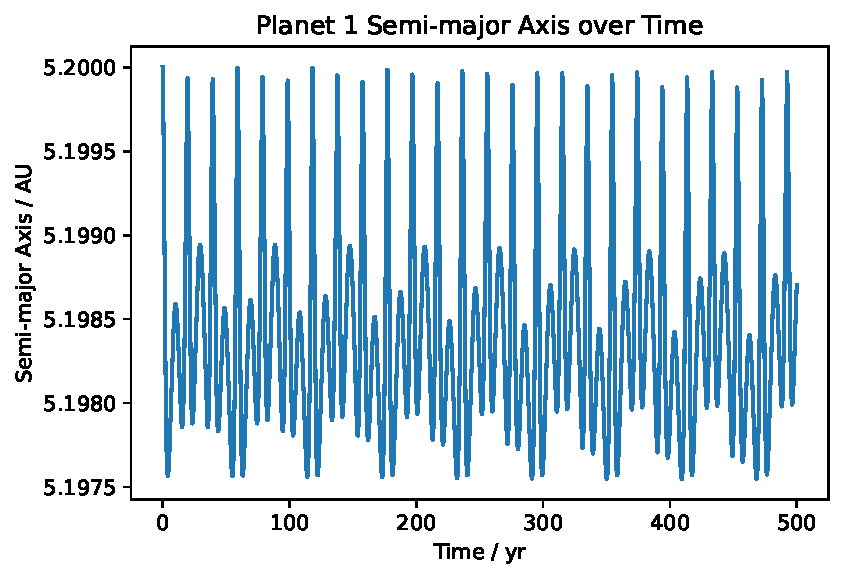
\includegraphics[width=0.6\textwidth]{q1f2.pdf}
    \captionsetup{justification=centering}
    \caption{The change in the semi-major axis of the orbit of Planet 1 as a function of time.}
    \label{fig:q1f2}
\end{figure}

Figure \ref{fig:q1f3} below shows the change in the semi-major axis for Planet 2, which exhibits similar oscillations, linked to those of Planet 1.

\begin{figure}[htp]
    \centering
    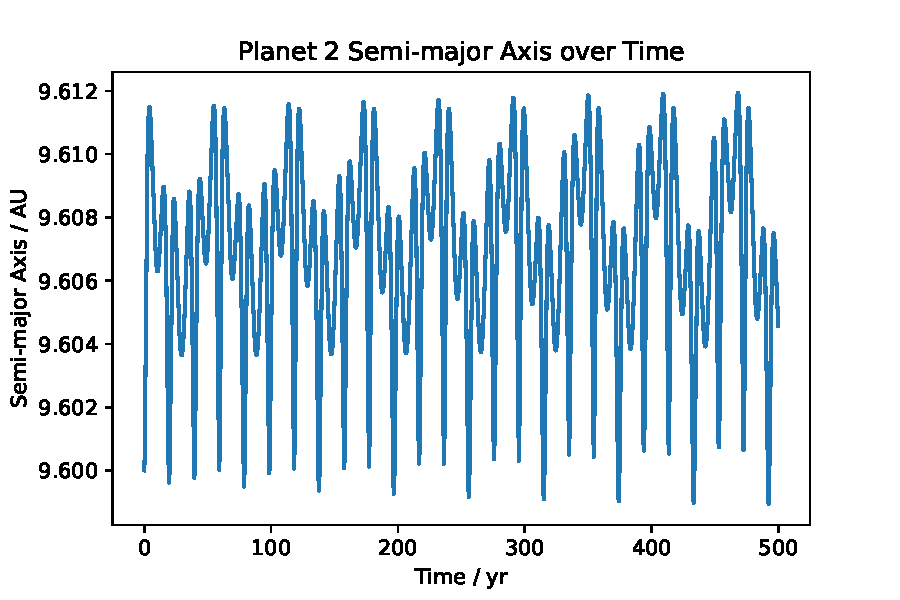
\includegraphics[width=0.6\textwidth]{q1f3.pdf}
    \captionsetup{justification=centering}
    \caption{The change in the semi-major axis of the orbit of Planet 2 as a function of time.}
    \label{fig:q1f3}
\end{figure}

\newpage

Figure \ref{fig:q1f4} below shows the evolution of the eccentricity of Planet 1 as a function of time. It also seems to oscillate at several concurrent frequencies due to interactions with the other bodies in the system, however on average it decreases with time during the specified time period.

\begin{figure}[htp]
    \centering
    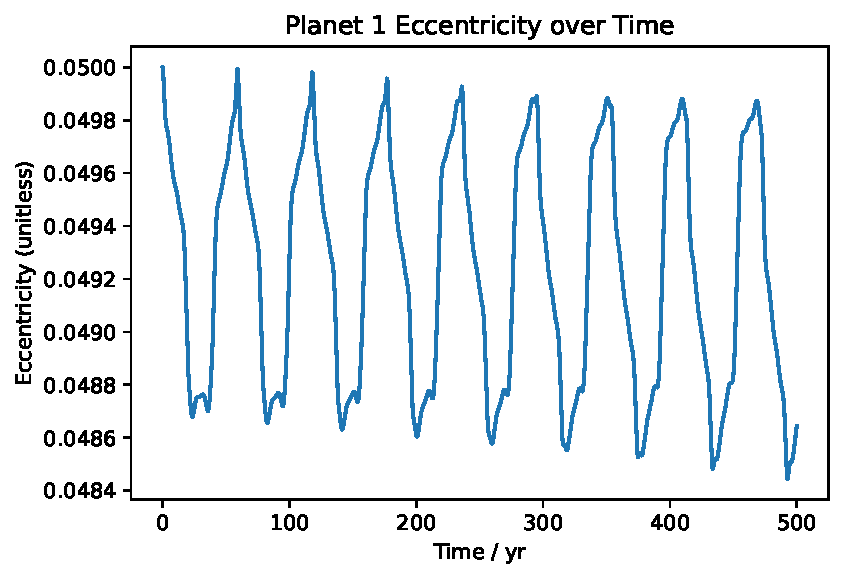
\includegraphics[width=0.6\textwidth]{q1f4.pdf}
    \captionsetup{justification=centering}
    \caption{The change in the eccentricity of the orbit of Planet 1 as a function of time.}
    \label{fig:q1f4}
\end{figure}

Figure \ref{fig:q1f5} below shows the change in the eccentricity of the orbit of Planet 2, which also oscillates but on average increases with time.

\begin{figure}[htp]
    \centering
    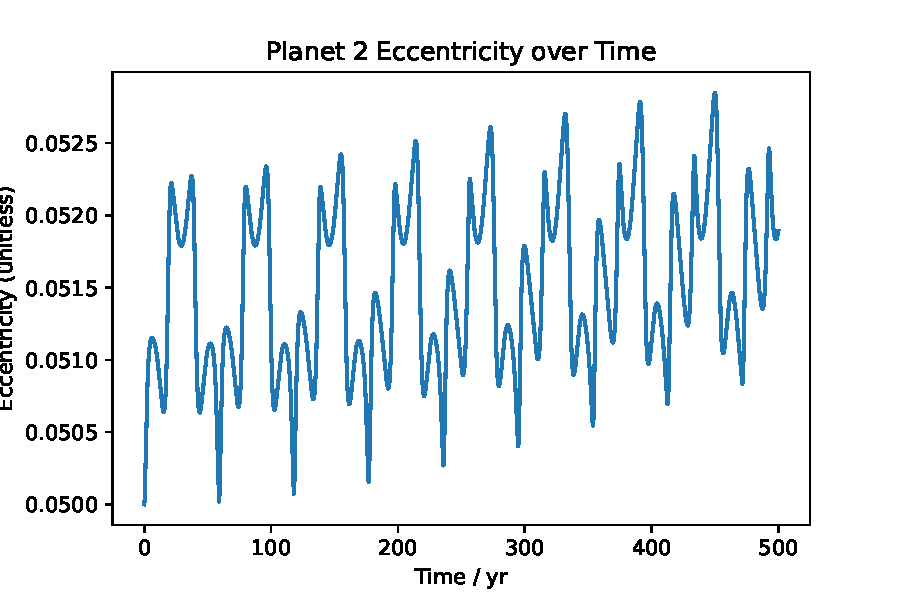
\includegraphics[width=0.6\textwidth]{q1f5.pdf}
    \captionsetup{justification=centering}
    \caption{The change in the eccentricity of the orbit of Planet 2 as a function of time.}
    \label{fig:q1f5}
\end{figure}

\newpage
%%%%%%%%%%%%%%%%%%%%%%%%%%%%%%%%%%%%%%%%%%%%%%%%%%%%%%%%%%%%%%%%%%%%%%%
\section{Making a Synthetic RV Curve and Understanding RV}

\subsection{}

We first define a function \simf{} which is used to run several, similar \rebound{} simulations with varying masses and orbital parameters, but the same number of planets, 1, and a single host star. This is particularly useful for the latter parts of this section since many simulations with varying parameters are conducted. \\
When called, the function creates a simulation which defaults to use the parameters given in part 1 of this section. Since each simulation is to be run for 30 orbits of the planet, but this orbit changes when parameters are modified, the period of orbit is calculated every time \simf{} is called, using the orbital elements calculations provided in the \rebound{} library. The total number of integration timesteps is set to 6000 such that each orbit contains 200 data points and meets the requirement of 10. Since all following parts only require information about the star's motion to calculate its radial velocity, the planets' orbital parameters are ignored in \simf{}. Thus only the star's x and y coordinates for each timestep are written to an array, and then its radial velocity is calculated at each timestep by dividing the change in x position between every two adjacent timesteps by the length of a timestep. This is a valid method of calculation because, for an observer on Earth, the distance to any star system is great enough that the angle between the line from Earth to the system and the velocity vector of the star when its movement is purely radial relative to Earth is negligible. The function returns a tuple containing the array of times and computed radial velocities of the star. \\

All following plots were generated by calling \simf{}, passing the modified parameter(s) or parameter ranges (in a \for{} loop) as specified. \\

\subsection{}
Figure \ref{fig:q2f1} shows that the radial velocity of the star changes with time, following a sinusoidal curve. The relatively slow motion of the star is attributed to its much larger mass compared to the planet. Since the planet's orbit was initilized with no eccentricity (and this is maintained nearly perfectly throughout the integration), we see that this sinusoidal motion in the x-direction arises because the planet and the star are both in circular motion about the barycentre of the system. 

\begin{figure}[htp]
    \centering
    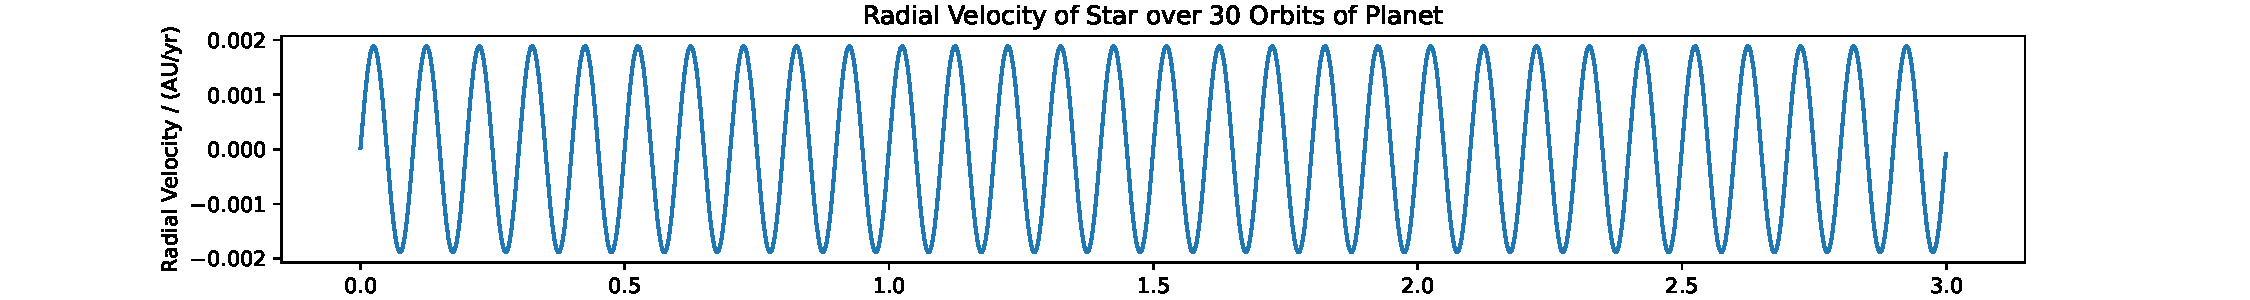
\includegraphics[width=0.95\textwidth]{q2f1.pdf}
    \captionsetup{justification=centering}
    \caption{The radial velocity, relative to a distant observer, of a star in a two-body system, with no eccentricity, over time.}
    \label{fig:q2f1}
\end{figure}

\subsection{}
Next we varied the stellar mass of the system, storing a range of values, and called \simf{} in a \for{} loop that iterated through these values. This produced the graph shown in Figure \ref{fig:q2f2} of the star's radial velocity with respect to time. 

\begin{figure}[htp]
    \centering
    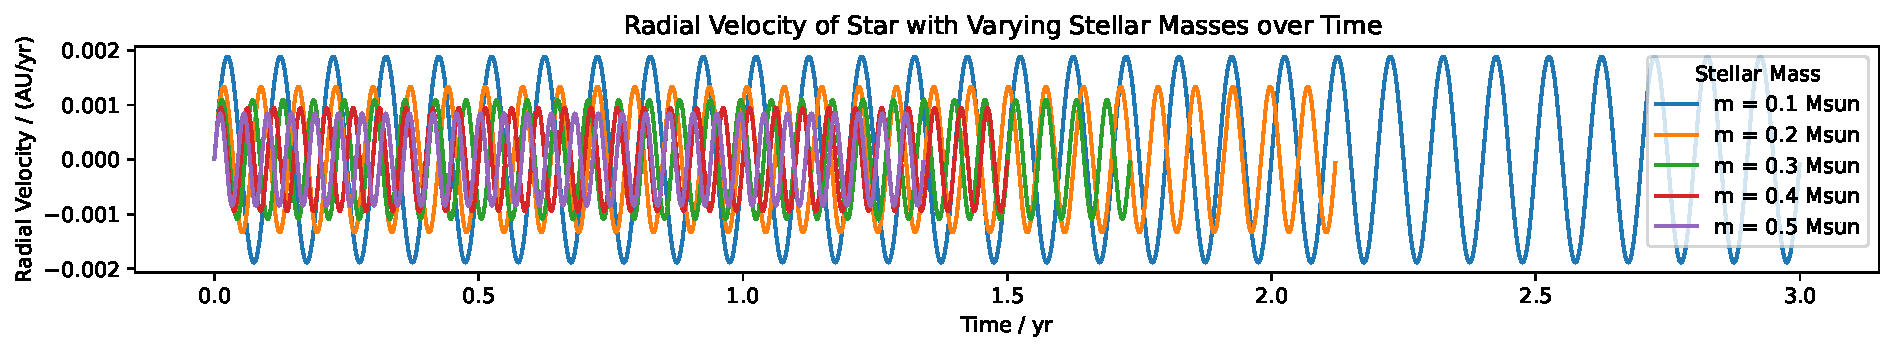
\includegraphics[width=0.95\textwidth]{q2f2.pdf}
    \captionsetup{justification=centering}
    \caption{The radial velocity of the star over time, varying only its mass.}
    \label{fig:q2f2}
\end{figure}

\newpage

Figure \ref{fig:q2f2} also conveys the impact of varying stellar mass on other properties of the system. We can see that the orbital period of the planet is inversely proportional to the square root of the mass of the star, thus the period of each oscillation in the curve is also inversely proportional to the square root of the star's mass. Moreover, the amplitude of each oscillation in radial velocity is inversely proportional to the square root of stellar mass. These observations are consistent with the equations of Newtonian Gravitation and uniform circular motion.  \\

We then varied the mass of the planet, in a similar fashion as before, calling \simf{} for each mass value used. Figure \ref{fig:q2f3} shows that the amplitude of oscillation of the radial velocity is directly proportional to the mass of the planet. 

\begin{figure}[htp]
    \centering
    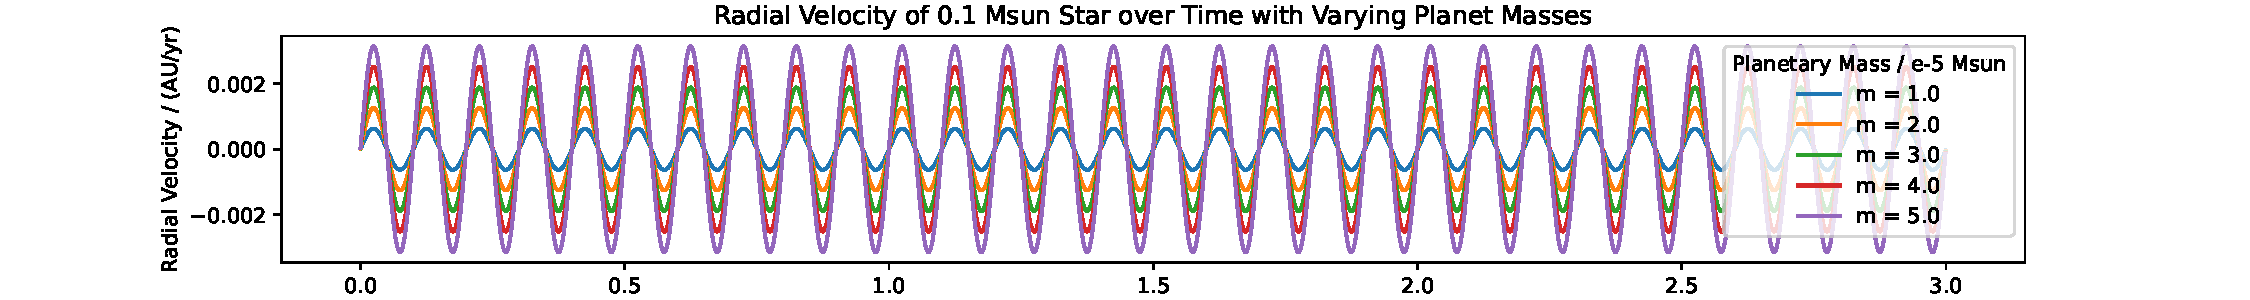
\includegraphics[width=0.95\textwidth]{q2f3.pdf}
    \captionsetup{justification=centering}
    \caption{The radial velocity of the star over time, varying only the planet's mass.}
    \label{fig:q2f3}
\end{figure}

This is because the magnitude of force between the two bodies is directly proportional to the mass of each body, and no other effects are seen because the mass of the star dominates the mass of the planet.\\

Next we varied the semi-major axis of the orbiting planet, running the simulations using \simf{} as before. Figure \ref{fig:q2f4} shows the results; the planet's (and thus star's) period is proportional to $a^{3/2}$ where $a$ is the planet's semi-major axis. Hence the period of oscillation of the star's radial velocity increases as the planet's semi-major axis increases, and its amplitude of oscillation decreases. These are again consistent with Newtonian and uniform circular motion equations. 

\begin{figure}[htp]
    \centering
    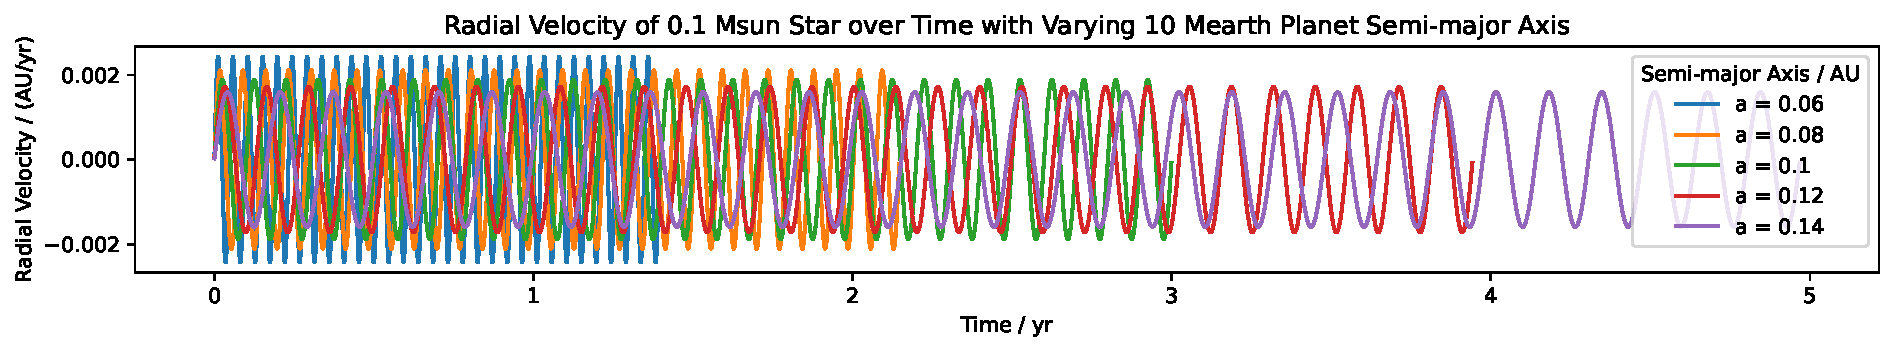
\includegraphics[width=0.95\textwidth]{q2f4.pdf}
    \captionsetup{justification=centering}
    \caption{The radial velocity of the star over time, varying only the planet's semi-major axis.}
    \label{fig:q2f4}
\end{figure}

\newpage

\subsection{}

We now rerun the simulation from section 2.1, but now passing in an eccentricity of $e = 0.3$ to \simf{}. Figure \ref{fig:q2f5} shows the results in years and AU/year, and Figure \ref{fig:q2f6} shows the same graph, instead in days and cm/s.

\begin{figure}[htp]
    \centering
    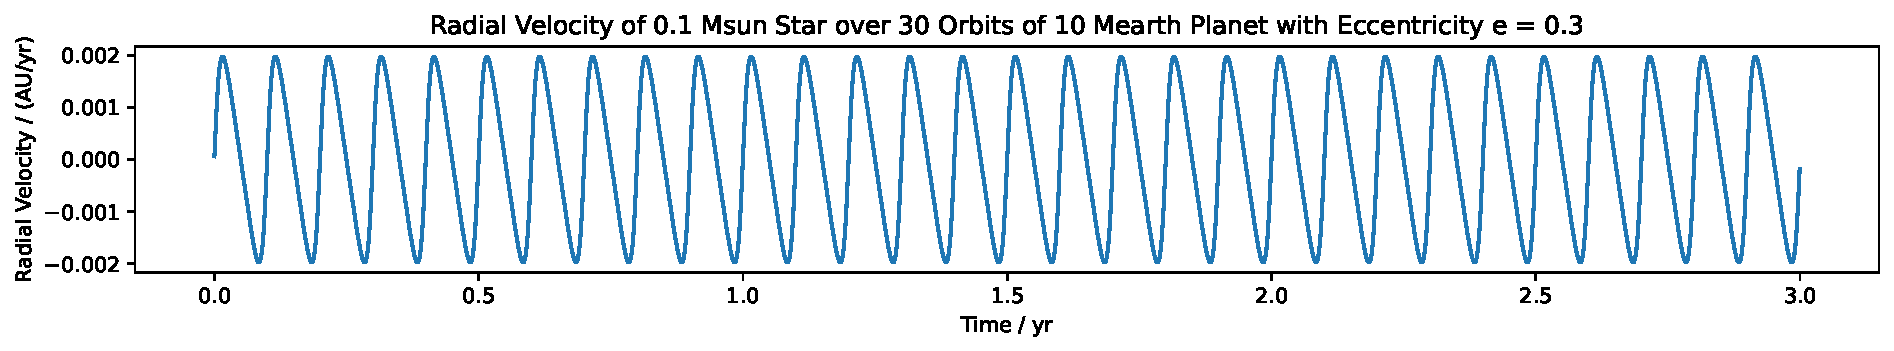
\includegraphics[width=0.95\textwidth]{q2f5.pdf}
    \captionsetup{justification=centering}
    \caption{The radial velocity of the star over time, with the planet having an orbital eccentricity of $e = 0.3$.}
    \label{fig:q2f5}
\end{figure}

\subsection{}

\begin{figure}[htp]
    \centering
    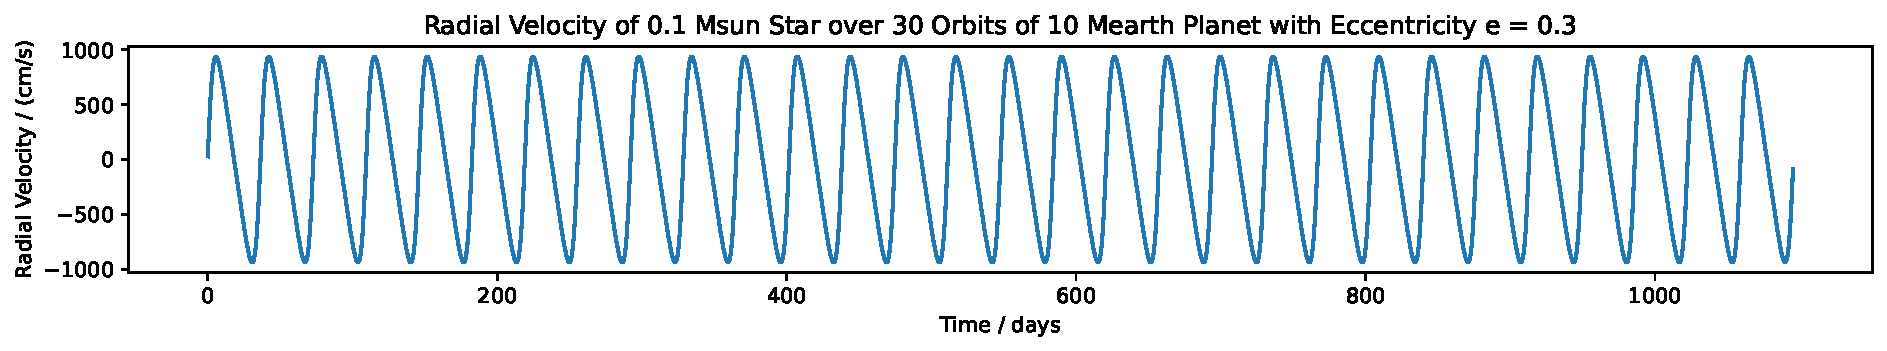
\includegraphics[width=0.95\textwidth]{q2f6.pdf}
    \captionsetup{justification=centering}
    \caption{The radial velocity of the star over time, with the planet having an orbital eccentricity of $e = 0.3$.}
    \label{fig:q2f6}
\end{figure}

We see that the resulting plot is very similar to Figure \ref{fig:q2f1}, with both graphs sharing almost the same maxima and minima. However, the graph is skewed, meaning that the rate of change of the radial velocity of the star is much greater when it is moving away from the observer compared to when it is moving towards the observer. This is because, although the trajectory of the planet in its elliptical orbit is symmetrical, it has a much higher velocity when it is near the star compared to when it is far away, which correlates to the skew seen in this figure. 

\newpage
%%%%%%%%%%%%%%%%%%%%%%%%%%%%%%%%%%%%%%%%%%%%%%%%%%%%%%%%%%%%%%%%%%%%%%%

\section{Fitting RV Data using \rebound{} and \texttt{emcee}}

\subsection{}

The data in the given file was first loaded into three arrays, as specified, using a \for{} loop. A plot was generated, shown in Figure \ref{fig:q3f1}.

\begin{figure}[htp]
    \centering
    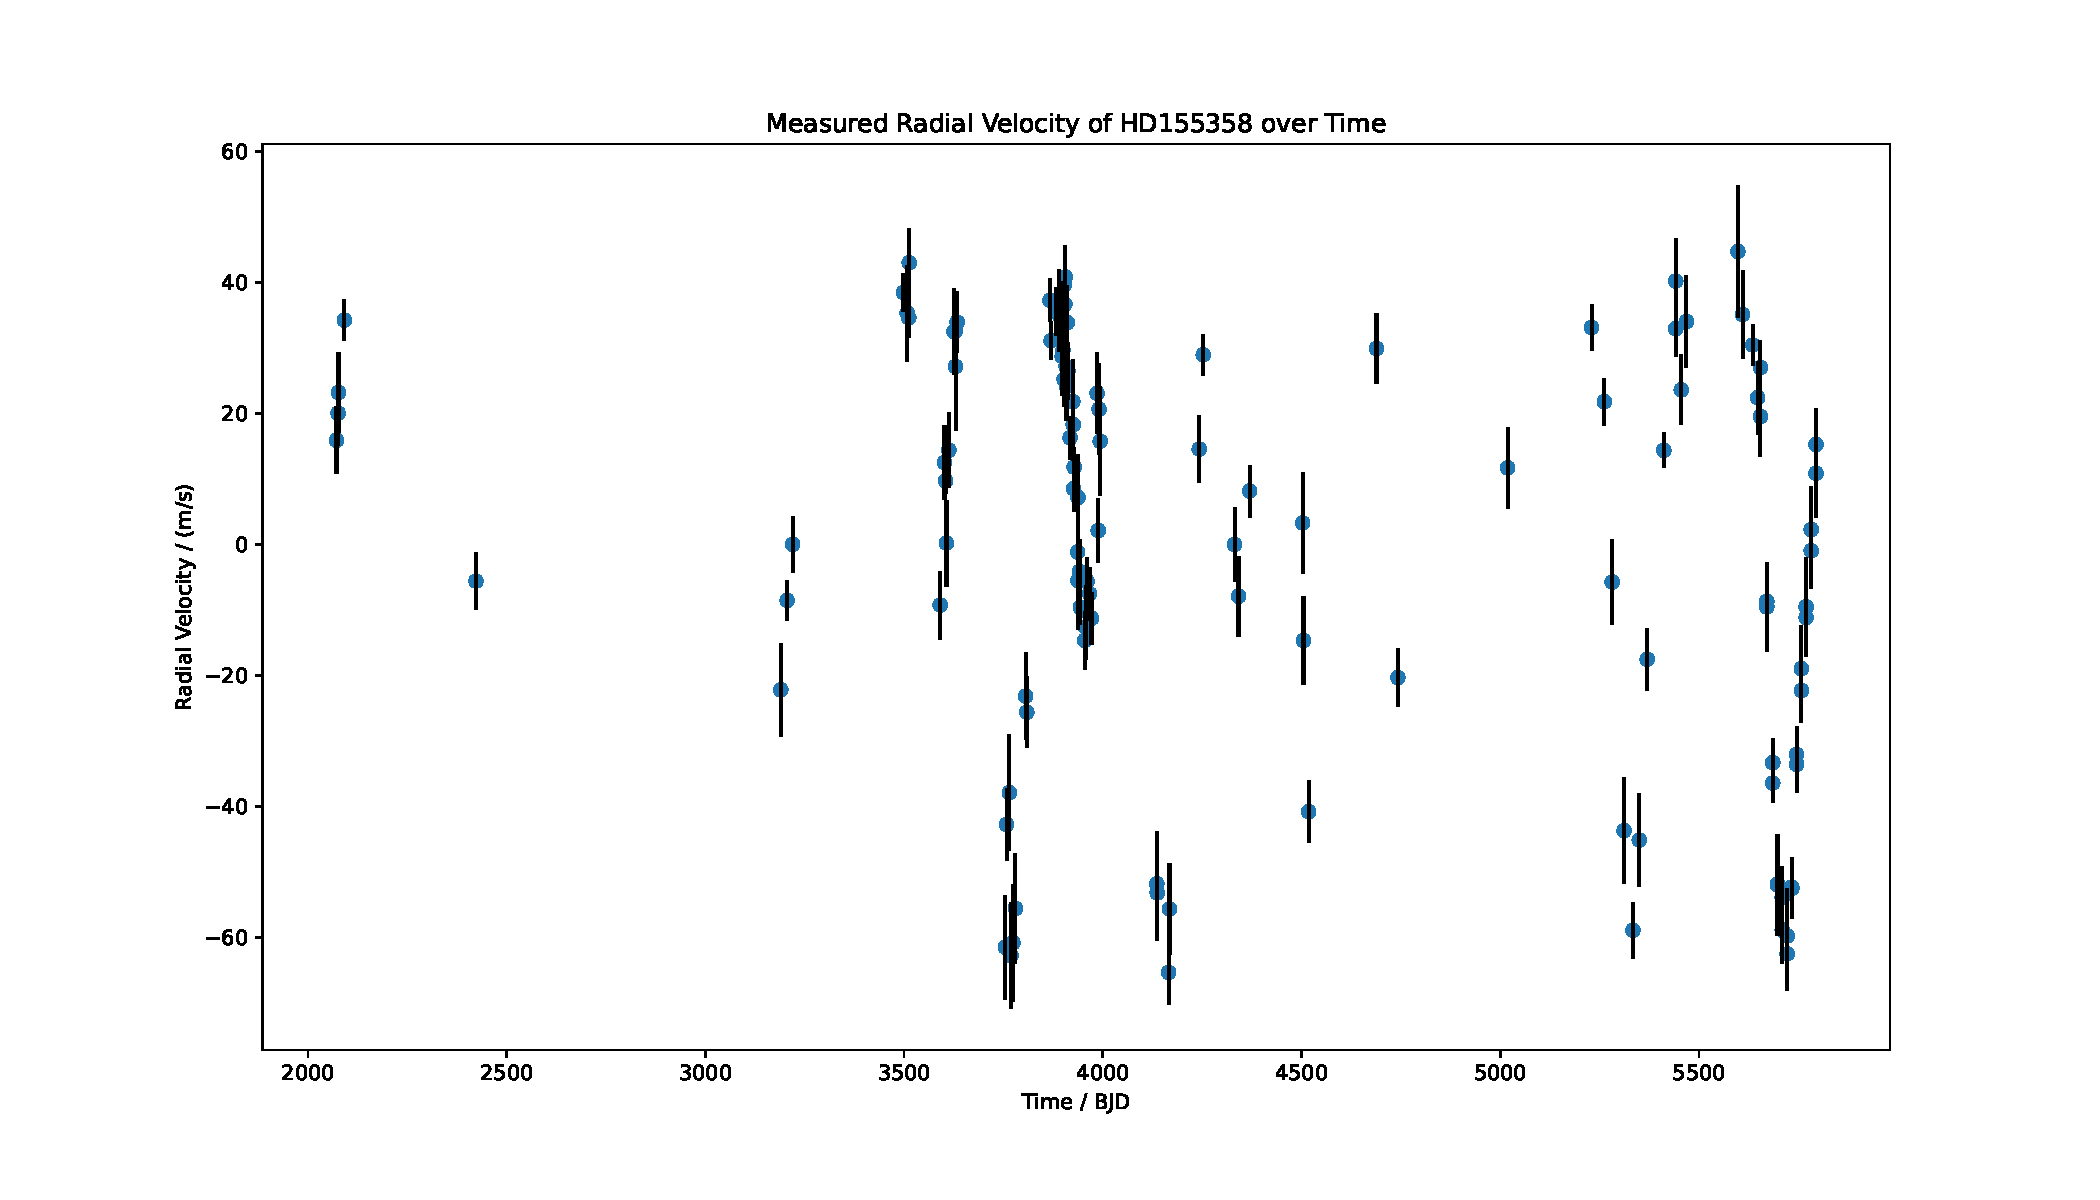
\includegraphics[width=0.95\textwidth]{q3f1.pdf}
    \captionsetup{justification=centering}
    \caption{The experimental values of the stellar radial velocity over time for the HD155358 system, suspected to have two Jovian planets.}
    \label{fig:q3f1}
\end{figure}

This appears to show two main periods during which most data was collected, occurring around 3800 BJD and 5700 BJD. Although the data seems to follow a steep piecewise curves in these regions, it is difficult to ascertain by eye a pattern followed by the data over the whole graph due to the sparse data points in most other regions. 

\newpage

\subsection{}

Next, a \rebound{} simulation was conducted using most of the code from within \simf{} with slight modifications (but without calling \simf{} directly), including the addition of one more planet. The system was created with the parameters specified in the PPI model in SR2017; specifically, with a star of mass $m = M_\odot$, a planet with mass $m_1 = 0.92 \si{M_J}$, semi-major axis $a_1 = 0.641 \si{AU}$, and eccentricity $e_1 = 0.17$, and a second planet with mass $m_2 = 0.85 \si{M_J}$, semi-major axis $a_2 = 1.017 \si{AU}$, and eccentricity $e_2 = 0.10$.\\
The simulation's start and end times as displayed in the plot shown in Figure \ref{fig:q3f2} were determined through trial and error. This is because at the time at which the planet's observations began, as in SR2017, the positions of the planets in the system did not match the default starting positions of planets in a \rebound{} simulation, thus the earliest such date where this was the case had to be found first in order to match the model to the given observational data.

\begin{figure}[htp]
    \centering
    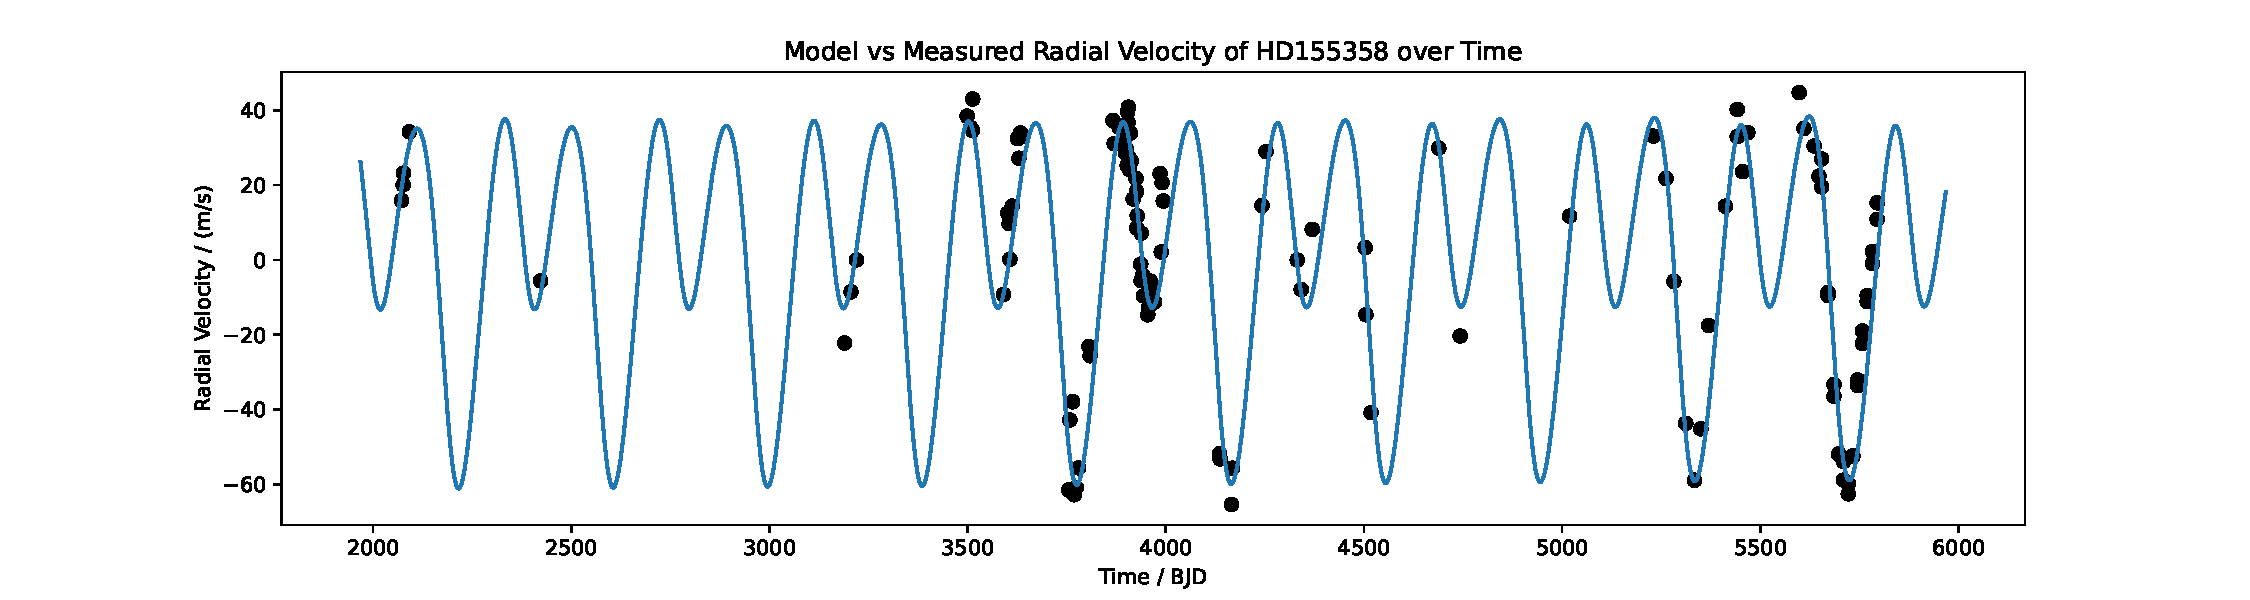
\includegraphics[width=0.95\textwidth]{q3f2.pdf}
    \captionsetup{justification=centering}
    \caption{The experimental values of the stellar radial velocity over time for the HD155358 system, superimposed on the model radial velocity curve.}
    \label{fig:q3f2}
\end{figure}

Overall, Figure \ref{fig:q3f2} resembles Figure 1 of SR2017 quite closely, thus showing a good fit of the model to real-life data.

%%%%%%%%%%%%%%%%%%%%%%%%%%%%%%%%%%%%%%%%%%%%%%%%%%%%%%%%%%%%%%%%%%%%%%%
\end{document}